\documentclass[12pt]{article} 
% \usepackage{amsfonts, amsmath, amssymb} 
\usepackage{dcolumn, multirow} 
\usepackage{setspace} 
\usepackage{epsfig, subfigure, subfloat, graphicx}
% \usepackage{booktabs}
\usepackage{tabularx} 
\usepackage{anysize, indentfirst, setspace} 
\usepackage{verbatim, rotating, paralist}
% \usepackage{pdfsync} 
\usepackage{latexsym} 
\usepackage{amsthm} 
\usepackage{fullpage} 
\usepackage{longtable} 
\usepackage{natbib} 
\usepackage{graphicx} 
\usepackage{mathabx} 
\usepackage{txfonts} 
%\usepackage{amsfonts} 
\usepackage{parskip} 
\usepackage{stmaryrd} 
%\usepackage{mathrsfs} 
% \usepackage{dsfont} 
\usepackage{comment} 
\usepackage{url} 
\usepackage{rotating} 
\usepackage{appendix}
\usepackage{booktabs}
% \usepackage{fontspec}
% \setmainfont{Baskerville}


\usepackage[margin=2.5cm]{geometry}

\title{The Effects of Ethnic Fractionalization on Market Efficiency: The Case of Rural Private Schools}
\author{Nick Eubank}
\date{\today}


\setcounter{tocdepth}{2}


% This is the beginning of a real document!
\begin{document} 
\maketitle

An often unstated assumption of market efficiency theorems is \emph{anonymity}: for markets to operate efficiently, different sellers offering the same good must be treated identically, at least from the perspective of a consumer. Yet in the ethnically fractionalized communities that characterize many rural developing villages today, it is not at all clear that this assumption is warranted. Rather, even in places where there are no clear hierarchies among ethnic groups, ethnic preferences can lead to socially segregated markets even within the same village, undermining competitive pressures and market efficiency. 

This paper illustrates the large effect that ethnic fragmentation can have on market efficiency in the context of private primary schools in rural Punjab, Pakistan. In recent years, rural private schools have come to be seen as a potential substitute for failing government schools, which have heretofore proven highly resistant to reform. Research has shown that in many contexts rural private schools radically outperform government schools, despite serving nearly nearly identical populations in terms of all available observables (wealth, parental education, etc.), and even after controlling for endogenous selection. Yet while this empirical regularity may hold generally, I show here that while private schools may dramatically outperform failing government schools in ethnically homogenous villages, this does not hold in more fractionalized contexts. Rather, I show that private schools are protected from the competitive pressures that would otherwise force them to produce better results to maintain enrollment by a reluctance of parents to send their children to other, less ``caste-appropriate'' schools in the village. As a result, not only does the ``private school premium'' (the difference between private and government test scores controlling for various observables) decline in highly fractionalized villages, but private schools are also able to charge higher fees despite their lower performance. 

This result is notable for a number of reasons. First, there is good reason to think that this result may be generalizable. Unlike in India -- where the most commonly known \emph{varna} caste system is hierarchical in nature -- castes in islamic societies like Pakistan have no general hierarchical ordering. The islamic system of castes (known as \emph{zaats}) more closely approximates a hereditary system of ``professional'' delineations. This makes lessons learned here potentially portable to other ethnically divided societies in places like sub-Saharan Africa (especially in other muslim societies with similar \emph{zaat} systems).

Second, it suggests a major new channel through which ethnolinguistic fractionalization (ELF) may lead to poor development outcomes. The relationship between ELF and violence, and ELF and low provision of public goods has been extensively documented, but to date the impact of ELF on \emph{market} outcomes has gone largely unstudied. Moreover, some have argued that markets act as substitutes for poor public good provision in high ELF societies, mitigating the negative effects of high ELF. Yet as shown here, this may be an optimistic interpretation -- while societies may sometimes turn to markets as a second best option when political systems fail to deliver public goods, this ``substitution'' is a very poor one, as ELF is as likely to disrupt markets as public provision. 

And third, it has important implications for policy in the educational sector. As previously noted, private schools are increasingly seen as viable substitutes for poor-performing and reform-resistant government schools in developing countries. This result suggests that such hopes may need to be tempered in ethnically fractionalized areas. 

The remainder of this research note is organized as follows. Section~\ref{data} provides a brief overview of the data used for this survey. Section~\ref{overview} provides an overview of the Pakistani context in which this study takes places, including a more detailed discussion of islamic castes, brief descriptives of the villages in the sample, and finally a discussion of segregation at the school level. Section~\ref{performance} presents evidence that segregation leads to poor market outcomes, including higher fees and lower performance by private schools. Section~\ref{alt} examines and rejects some alternative explanations for the empirical patterns presented. Section~\ref{india} provides a brief note on plans to test the generalizability of this finding with data from India (including some preliminary results), and finally Section~\ref{problems} details some of the outstanding problems with the preceding analysis. 


\section{Data}\label{data}

This analysis is based on data from the Learning and Educational Attainment in Punjab Schools (LEAPS) survey conducted from 2003-2007. The survey provides both cross-section and panel data on schools, teachers, households, and students from over one hundred villages in rural Punjab, Pakistan. Villages were selected from a universe of all villages with at least one private school on a PPS basis. The sample was also stratified across three districts. In all, LEAPS sample consists of more than 800 schools from 112 rural villages, balanced evenly across three districts. 

Central to the survey are a set of exams, administered by the LEAPS team, in urdu, math, and english. These exams were administered to some 30,000 students in every government and private school in sample villages over the four year survey. These results were then used to generated standardized test scores for all students using Item Response Theory. All scores reported here have a mean of zero and a standard deviation one at grade 3. 

\section{The Context}\label{overview}

\subsection{Islamic Caste System}\label{}

As noted in the introduction, the focus of this paper is on ethnic fractionalization measured by the islamic caste system. Castes in islamic societies (usually referred to as \emph{zaats}) do not fit into a general hierarchy as in other countries, but are more like ethnic categories found in many African countries, where ethnic groups may hold different relative social positions in different villages. Some \emph{zaats} are religious (like Sheikhs), while others are more like historical occupational groupings (for example, lohars are historic iron workers). These castes are also highly diverse -- this analysis includes more than 20 categories of \emph{zaat}.\footnote{The indian equivalent of zaats are \emph{jatis}, which have a similar structure. Unlike \emph{varnas}, \emph{jatis} in India do not have a strict hierarchy. It is also interesting to note that some historians argue that the current hierarchical system of \emph{varnas} is essentially the creation of the british, who preferred a simple taxonomy of social status to the more complicated system of \emph{jatis} that prevailed upon their arrival.}

The multiplicity of castes and the lack of a general hierarchy makes analysis of caste politics somewhat difficult. For example, it precludes a simple analysis of where high and low castes attend school. One possible future route for research is to estimate a caste hierarchy within each village based on land holdings, but some \emph{zaats} who tend to be of relatively ``high status'' explicitly avoid holding land (like Syeds).\footnote{Jacoby and Mansuri have attempted this with mixed success.}

\subsection{Villages}\label{}

Villages in Punjab represent surprisingly competitive educational market places -- the typical village in the LEAPS survey has 8 primary schools. Moreover, these schools are often densely clustered -- the average private school is located such that \emph{half} of all other schools in the village are within a five minute walk, and less than a third are more than 15 minutes away. LEAPS data shows that parents -- even illiterate and uneducated parents -- have a very good understanding of the quality of schools in their village, a crucial ingredient for competitiveness, and in most cases private schools are highly affordable. As a result, private schools serve a very similar population to government schools: private school students are slightly wealthier on average, but the distributions overlap tremendously, as shown below in Figure~\ref{wealthdist}. 


\begin{figure}[htb]
	\begin{center}
	\caption{}\label{wealthdist}
	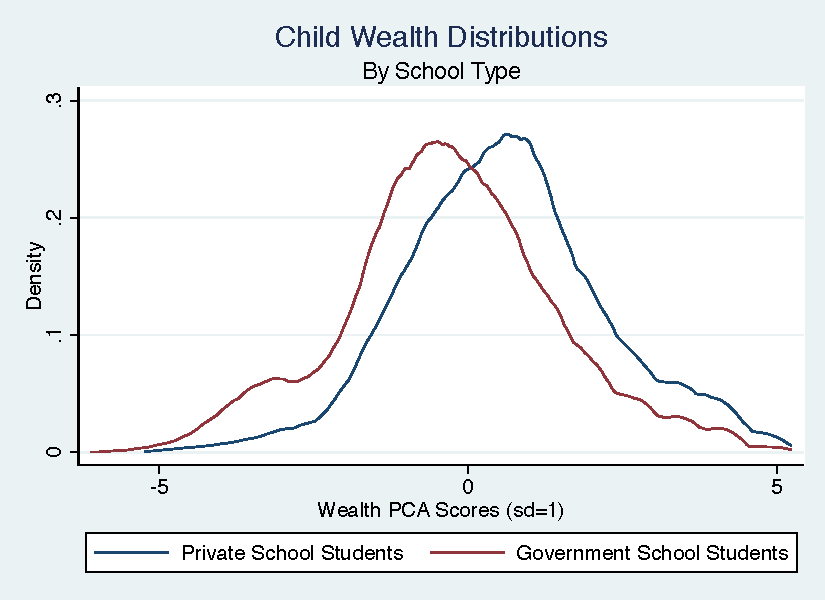
\includegraphics[scale=1.0]{graphs/wealth_and_type.pdf}
	\end{center}
\end{figure}


Despite serving similar populations, private school students massively outperform their government school counterparts. At Class 3, private school students are approximately a year and a half ahead government school students in math, urdu, and english. Although it is outside the scope of this note, the general conclusion of the LEAPS authors is that this performance is due largely to more attentive teaching and private school responses to competitive pressures, rather than selection. 

Villages also vary dramatically in their ethnic composition. Figure~\ref{fracdensities} below shows the density plot of villages of different levels of ethnic fractionalization, which is computed as a simple herfindahl index of \emph{zaats}.\footnote{Note that this measure was computed not on the basis of LEAPS survey results, but the household listing census completed in 2002 (the LEAPS survey includes only 10 households per villages, so the listing census likely provides a much more accurate measure of fractionalization).} As the figure shows, there is significant heterogeneity in the degree of fractionalization across villages, and across districts. Careful attention is given to ensuring results are not driven by cross-district differences at all times.

\begin{figure}[htb]
	\begin{center}
	\caption{}\label{fracdensities}
	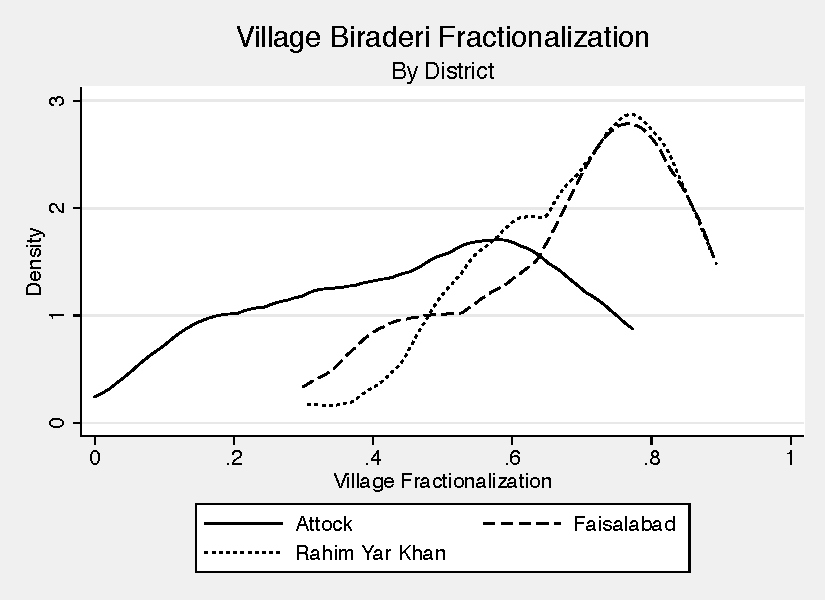
\includegraphics[scale=1.0]{graphs/village_frac_by_district.pdf}
	\end{center}
\end{figure}


One note: I have continued to use this herfindahl measure linearly in all analyses, but I'm not convinced this is appropriate. Linearity implies that a village with a score of 0.6 is ``twice'' as fractionalized as a village with a score of 0.3.  My own sense is that given how the measure is calculated, a move from 0.6 to 0.9 is a much bigger shift than from 0.3 to 0.6, especially when working with so many categories (recall there are more than 20 caste groups). Indeed, in all my results, and those I have looked at in other countries, the bulk of village observations are in the 0.6 to 0.9 range, and yet look quite different from one another qualitatively. I am hesitant to make any direct modifications to the measure for fear of accusations of ``data-mining'', but if you know of any literature that would justify this kind of adjustment I would greatly appreciate it. 


Interestingly, segregation is not clearly related to any other village characteristics, as shown below in Table~\ref{vsummary}. Nor is this lack of clear relationship driven by district differences -- as shown in Table~\ref{vsummarydemeaned}, in which summary statistics are computed after demeaning values for district averages. Please note that ``high,'' ``medium'' and ``low'' fractionalization in these tables refer to village fractionalization terciles, as they whenever these categories are used in this paper. 

% matrix: results file: /Users/Nick/dropbox/data/LEAPS/data//constructed/ethnic_info/docs/tables/village_summary.tex   2 Sep 2012 21:28:58
\begin{table}[htbp]
\caption{\label{vsummary} Village Summary Statistics}\centering\medskip
\begin{tabular}{|l|l|l|l|l|l|}\hline  
 & Median Expend  & Adult Lit Rate  & Pct Enrollment  & Schools per HH  & Num Households  \\ \hline  
Highest Frac &      4967 &        39 &        70 &      .017 &       699 \\ \hline 
Moderate Frac &      4194 &        34 &        67 &      .019 &       631 \\ \hline 
Lowest Fract &      4719 &        38 &        75 &      .011 &       562 \\ \hline 
All &      4641 &        37 &        71 &      .016 &       631 \\ \hline 
  \end{tabular}
\end{table}

% matrix: results file: /Users/Nick/dropbox/data/LEAPS/data//constructed/ethnic_info/docs/tables/village_summary_demeaned.tex   2 Sep 2012 21:29:00
\begin{table}[htbp]
\caption{\label{vsummarydemeaned} Summary Statistics, After Subracting District Averages}\centering\medskip
\begin{tabular}{|l|l|l|l|l|l|}\hline  
 & Median Expend  & Adult Lit Rate  & Pct Enrollment  & Schools per HH  & Num Households  \\ \hline  
Highest Frac &       1.2 &      -.17 &        -1 &     .0019 &        65 \\ \hline 
Moderate Frac &        19 &      -.51 &         1 &    .00041 &       1.4 \\ \hline 
Lowest Fract &       -19 &       .65 &       .12 &    -.0023 &       -68 \\ \hline 
All &  -3.3e-06 &   9.2e-08 &  -1.3e-07 &  -1.3e-11 &  -9.1e-07 \\ \hline 
  \end{tabular}
\end{table}




\subsection{Segregation}\label{}

Of critical importance to my argument is that schools in highly fractionalized villages are segregated. As noted above, because of the sheer number of non-hierarchical castes, showing this is non-trivial. Below I present three pieces of evidence I believe support the argument that castes are indeed highly segregated across schools. 

First, if schools were unsegregated, one would naturally expect the number of castes present in a school to be higher in more fractionalized villages than in more homogenous villages. Yet as shown in Figure~\ref{numcastes}, this is not the case -- the number of castes represented in a school has nearly the same distribution in highly fractionalized villages and in less fractionalized villages. 


\begin{figure}[H]
	\begin{center}
	\caption{}\label{numcastes}
	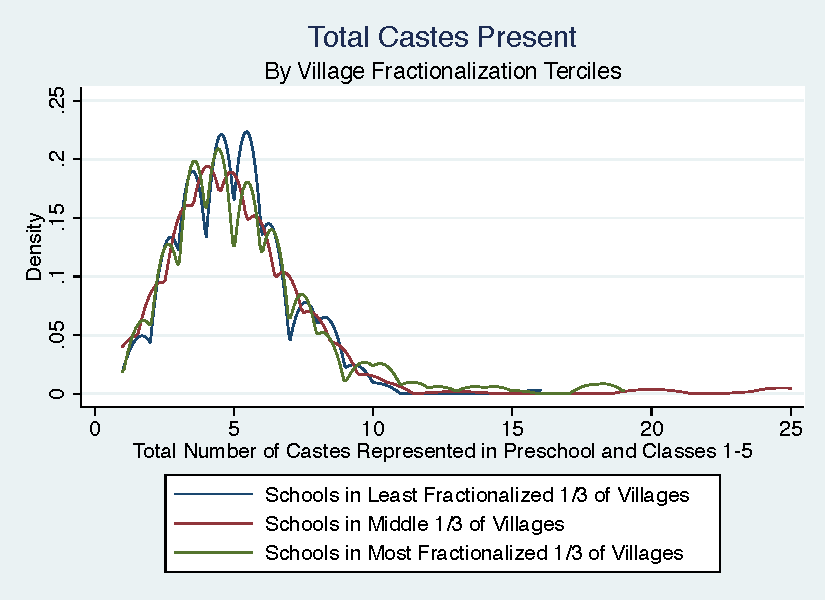
\includegraphics[scale=1.0]{graphs/totalpresent.pdf}
	\end{center}
\end{figure}


Second, let us consider the share of population made up of the largest two castes in a village. In more fractionalized villages, of course, this share is lower, and indeed this is what we see in Figure~\ref{villagetoptwo}. Yet as shown in Figure~\ref{schooltoptwo}, this does not hold for \emph{schools} to nearly the same degree. In more fractionalized villages the share of students from the top two castes in the average school is indeed slightly lower, but not by nearly as much as suggested by the change in village demographics.

\begin{figure}[H]
	\begin{center}
			\caption{Villages}\label{villagetoptwo}
			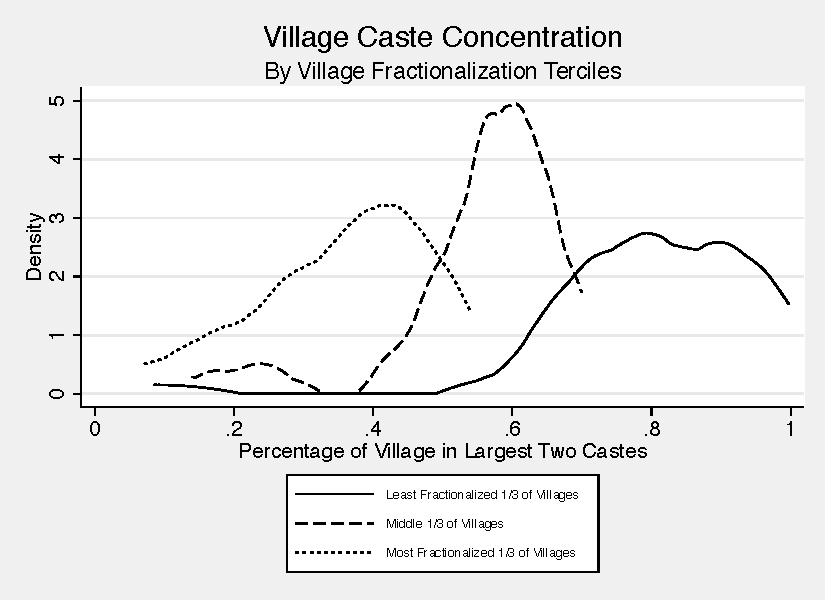
\includegraphics[scale=1]{graphs/village_toptwo.pdf}\caption{Schools}\label{schooltoptwo}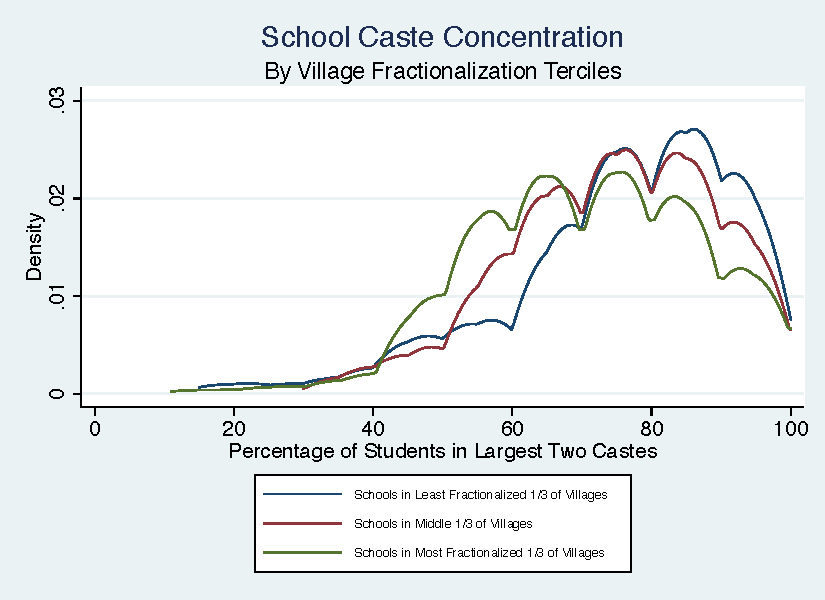
\includegraphics[scale=1]{graphs/school_toptwo.pdf}
	\end{center}
\end{figure}


And finally, if schools are unsegregated, then we would expected herfindahl indices computed within each school to track closely with herfindahl indices computed at the village level. Yet as shown in Figure~\ref{schoolvvillageherf}, this is far from the case. Almost all schools are below the 45 degree line that would indicate school and village diversity moving one for one, and many are well below. 


\begin{figure}[H]
	\begin{center}
	\caption{}\label{schoolvvillageherf}
	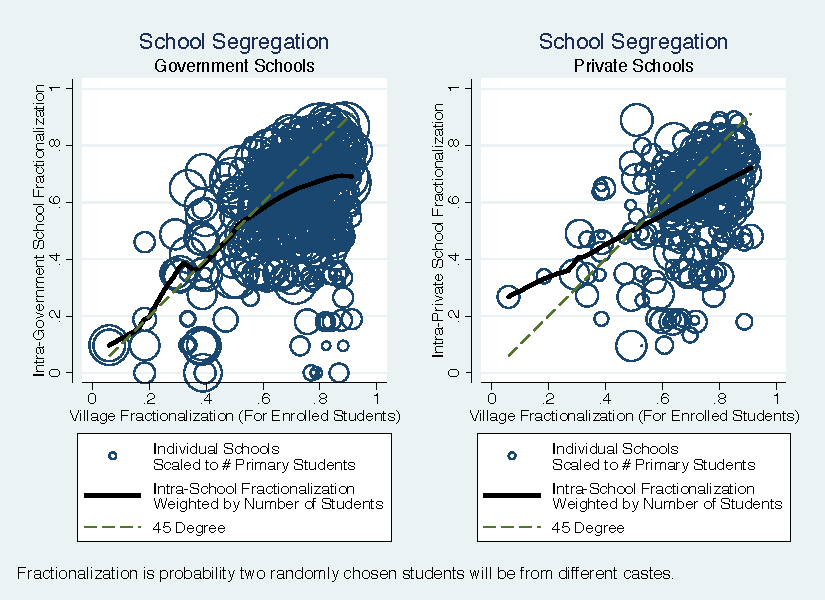
\includegraphics[scale=1.0]{graphs/intra_versus_intervillage_frac_combined.pdf}
	\end{center}
\end{figure}

\pagebreak
\pagebreak

\section{Segregation and Private School Performance}\label{performance}
As shown above, schools in fractionalized villages appear to be highly segregated, suggesting immobility of students between schools. The argument of this paper is that this immobility impedes the competitive pressure faced by schools. This ``diminished pressure'' is evident in two patterns. First, private schools in highly fractionalized villages charge \emph{dramatically} higher fees than those in less fractionalized villages, even when controlling for things like village wealth. And second, the test score ``premium'' private schools offer over government schools is dramatically lower in highly fractionalized villages than in homogenous villages, even when controlling for things like parental education, family wealth, etc. Yet despite the fact that private schools offer less and charge more, private school enrollment rates are nearly the same in these villages as in more homogenous villages (as shown in Table~\ref{privateshare}), suggesting that private schools are less competitive, and to some degree are substituting segregation for education in their sales pitches.

\begin{table}[htbp]\centering
\def\sym#1{\ifmmode^{#1}\else\(^{#1}\)\fi}
\caption{Share of Enrolled Students in Private Schools \label{privateshare}}
\begin{tabular}{l*{2}{c}}
\toprule
                &\multicolumn{1}{c}{(1)}&\multicolumn{1}{c}{(2)}\\
                &\multicolumn{1}{c}{Share Students in Private School}&\multicolumn{1}{c}{Share Students in Private School}\\
\midrule
Biraderi Fractionalization&    0.077   &    0.085   \\
                &  (0.060)   &  (0.032)   \\
Median Village Expenditure&            & 0.000029** \\
                &            &(0.0000040)   \\
Village Land Gini&            &    0.022   \\
                &            &  (0.087)   \\
Village: Pct Adults Literate&            &   0.0019   \\
                &            & (0.0019)   \\
Log Num HHs     &            &    0.019   \\
                &            &  (0.022)   \\
District Fixed Effects&      Yes   &      Yes   \\
\midrule
Observations    &      112   &      112   \\
\bottomrule
\multicolumn{3}{l}{\footnotesize Standard errors in parentheses}\\
\multicolumn{3}{l}{\footnotesize * \(p<0.10\), ** \(p<0.05\), *** \(p<0.01\)}\\
\multicolumn{3}{l}{\footnotesize Results clustered at district level.}\\
\end{tabular}
\end{table}



\subsection{Private School Fees}\label{}

Despite offering a much smaller performance premium over government schools in the same village, private schools in ethnically fractionalized villages charge dramatically more than private schools in homogenous villages. As shown in Table~\ref{fees} below, moving from a perfectly non-fractionalized village to a perfectly fractionalized village is associated with a 600 Rupees increase in annual school fees. Given that the average annual fee for all private schools in the LEAPS survey is 1191 Rupees, this is a very significant amount.\footnote{Fees above the 95th percentile -- 1900 Rupees -- were adjusted down to 1900 Rupees. Without this adjustment, the coefficient on village fractionalization is approximately 950 Rupees with a t-stat of 2.09} 

\begin{table}[htbp]\centering
\def\sym#1{\ifmmode^{#1}\else\(^{#1}\)\fi}
\caption{Annual Private School Fees\label{fees}}
\begin{tabular}{l*{3}{c}}
\toprule
                &\multicolumn{1}{c}{(1)}&\multicolumn{1}{c}{(2)}&\multicolumn{1}{c}{(3)}\\
                &\multicolumn{1}{c}{Weighted by School}&\multicolumn{1}{c}{Weighted by School}&\multicolumn{1}{c}{Weighted by Primary Students}\\
\midrule
Biraderi        &    504.7** &    527.9** &    608.6** \\
Fractionalization&   (2.33)   &   (2.50)   &   (2.37)   \\
Village: Median &            &     61.6   &     20.8   \\
Expenditures    &            &   (1.25)   &   (0.44)   \\
Expenditure Gini&            &    -49.9   &     45.5   \\
                &            &  (-0.24)   &   (0.20)   \\
District Fixed Effects &      Yes   &      Yes   &      Yes   \\
\midrule
Observations    &      287   &      287   &      285   \\
\bottomrule
\multicolumn{4}{l}{\footnotesize \textit{t} statistics in parentheses}\\
\multicolumn{4}{l}{\footnotesize * p<0.10, ** p<0.05, *** p<0.01}\\
\end{tabular}
\end{table}



Yet despite these radically higher fees, if anything a \emph{higher} share of enrolled students are in private schools in fractionalized villages, as shown in Table~\ref{privateshare}. 


\subsection{Private School Educational Premium}\label{}
In addition to charging more, private schools in more fractionalized villages also deliver less in terms of their superiority to government schools in the same village. Showing this is obviously complicated, as computing the contribution of a school to a child's testscores is non-trivial. With that in mind, the results of three different methods of measurement are presented here, each of which has different strengths and weaknesses, but all of which show a consistent picture of lower relative private school performance in highly fractionalized villages. 

\subsubsection{Cross-Sectional Test Scores}\label{} 

The first presentation of results uses cross-sectional test scores. This approach provides results based on the largest sample sizes available -- 17,670 children in Class 3 with limited controls, and 9,386 children with more extensive controls. Examining level differences rather than the magnitude of change over time (what we traditionally think of as learning) is clearly a second best option, but given that students do not appear to change schools with great frequency and we are examining children at the start of their educational career, level differences between government and private students are likely a better reflection of the differences in school systems than they would be if we were comparing levels at a secondary school level.

Using this cross-sectional approach, Figure~\ref{crosssectiongraphs} shows the ``private school test premium'' (the difference between government and private test scores controlling for various observable child characteristics and village fixed effects) for all three subjects. In all three subjects, private school premiums decrease dramatically with ethnic fractionalization (the underlying regressions for which are presented in Table~\ref{crosssection}).

\begin{figure}[htb]
	\caption{Private School Test Score Premium}\label{crosssectiongraphs}
	\centering	
	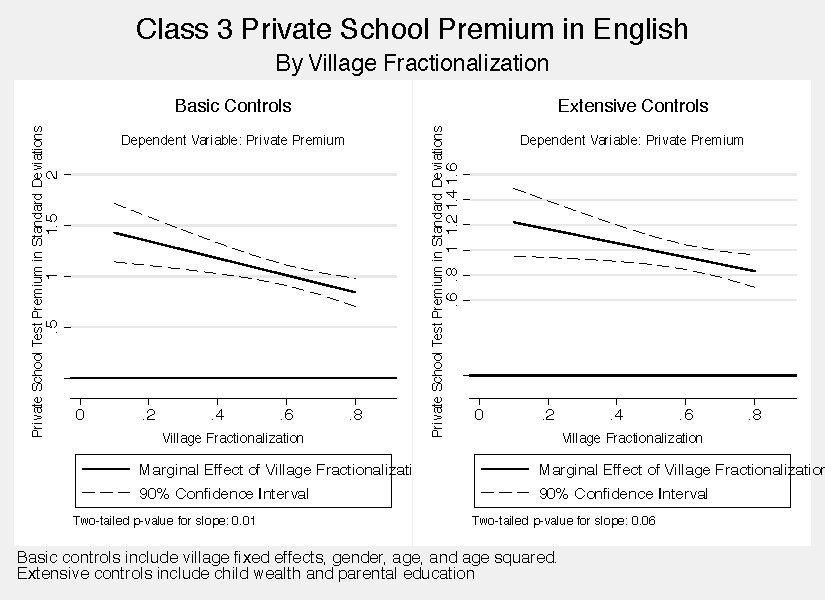
\includegraphics[scale=0.8]{graphs/privatepremium_english_crosssection.pdf}
	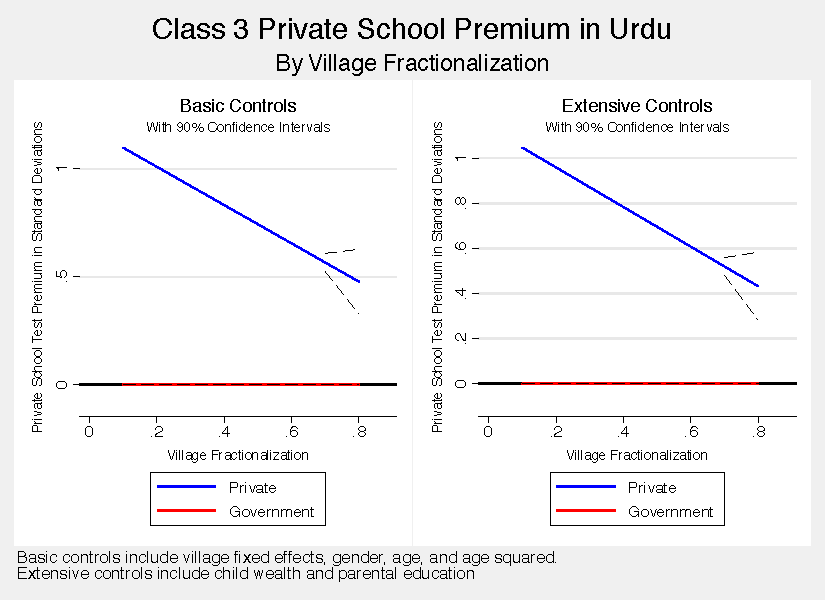
\includegraphics[scale=0.8]{graphs/privatepremium_urdu_crosssection.pdf}
	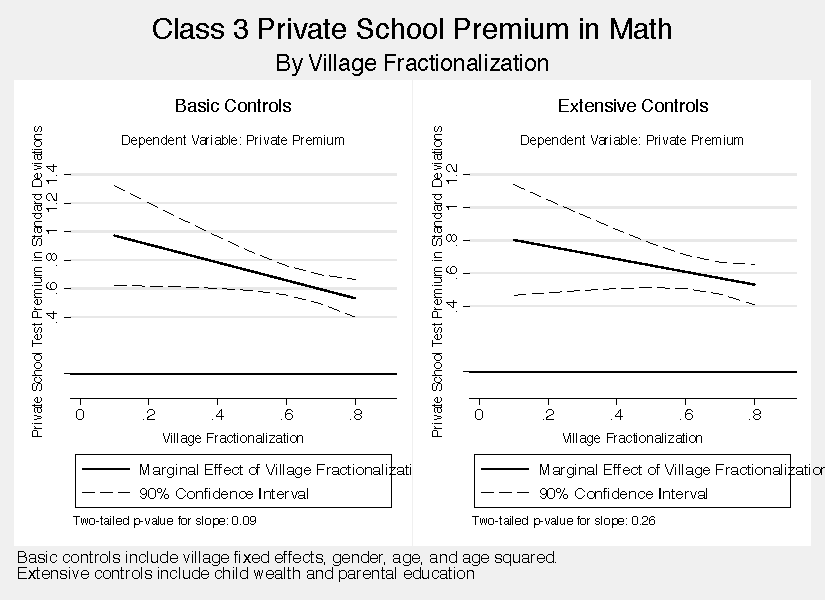
\includegraphics[scale=0.8]{graphs/privatepremium_math_crosssection.pdf}
\end{figure}

\begin{table}[htbp]\centering
\def\sym#1{\ifmmode^{#1}\else\(^{#1}\)\fi}
\caption{Class 3 Cross-Sectional Private School Premium\label{crosssection}}
\begin{tabular}{l*{6}{c}}
\toprule
                &\multicolumn{2}{c}{English}&\multicolumn{2}{c}{Urdu} &\multicolumn{2}{c}{Math} \\\cmidrule(lr){2-3}\cmidrule(lr){4-5}\cmidrule(lr){6-7}
                &\multicolumn{1}{c}{(1)}&\multicolumn{1}{c}{(2)}&\multicolumn{1}{c}{(3)}&\multicolumn{1}{c}{(4)}&\multicolumn{1}{c}{(5)}&\multicolumn{1}{c}{(6)}\\
                &\multicolumn{1}{c}{}&\multicolumn{1}{c}{}&\multicolumn{1}{c}{}&\multicolumn{1}{c}{}&\multicolumn{1}{c}{}&\multicolumn{1}{c}{}\\
\midrule
Private School  &     1.39***&     1.26***&     0.96***&     0.89***&     0.91***&     0.84***\\
                &   (9.59)   &   (8.78)   &   (7.98)   &   (7.03)   &   (5.68)   &   (5.29)   \\
Zaat-Private Interaction&    -0.72***&    -0.60***&    -0.47** &    -0.42** &    -0.41   &    -0.33   \\
                &  (-3.14)   &  (-2.73)   &  (-2.40)   &  (-2.10)   &  (-1.57)   &  (-1.33)   \\
Female          &     0.19***&     0.16***&     0.18***&     0.18***&   -0.081*  &   -0.090** \\
                &   (5.11)   &   (4.79)   &   (5.10)   &   (6.12)   &  (-1.75)   &  (-2.34)   \\
Child Age       &    0.049   &    0.049   &    0.030   &    0.043   &     0.10** &     0.11** \\
                &   (1.57)   &   (1.34)   &   (0.84)   &   (1.04)   &   (2.24)   &   (2.16)   \\
Age Squared     &  -0.0029*  &  -0.0027   &  -0.0015   &  -0.0022   &  -0.0041*  &  -0.0045*  \\
                &  (-1.95)   &  (-1.55)   &  (-0.87)   &  (-1.10)   &  (-1.87)   &  (-1.76)   \\
Child's Wealth Index&            &    0.040***&            &    0.022***&            &    0.013*  \\
                &            &   (6.69)   &            &   (3.45)   &            &   (1.82)   \\
Educated Parent &            &    0.095***&            &    0.092***&            &    0.080***\\
                &            &   (4.68)   &            &   (4.09)   &            &   (3.19)   \\
Village Fixed Effects&      Yes   &      Yes   &      Yes   &      Yes   &      Yes   &      Yes   \\
\midrule
Observations    &    23681   &    12545   &    23681   &    12545   &    23681   &    12545   \\
\bottomrule
\multicolumn{7}{l}{\footnotesize \textit{t} statistics in parentheses}\\
\multicolumn{7}{l}{\footnotesize * p<0.10, ** p<0.05, *** p<0.01}\\
\end{tabular}
\end{table}


\subsubsection{Test Scores with Lagged Scores}\label{} 
A second approach is to examine a cross-section of test scores with lagged scores as an additional control. Although clearly a superior technique for measuring the contribution of a school in a year, it can only be applied in one half of the villages in the LEAPS sample.\footnote{The LEAPS survey included a randomized intervention starting in Year 2 of the survey that I believe may have had a differential effect on high and low fractionalization villages. Treated villages must therefore be excluded after Year 1, which precludes looking at panel patterns in treated villages.} Nevertheless, these results are quite consistent with those from above. Figure~\ref{withlags} shows the private school premium at Class 4 controlling for Class 3 scores. Again, the results are both large and significant, as confirmed by Table~\ref{wlags}.

\begin{figure}[h]
	\caption{Private School Test Score Premium with Lagged Scores}\label{withlags}
	\centering	
	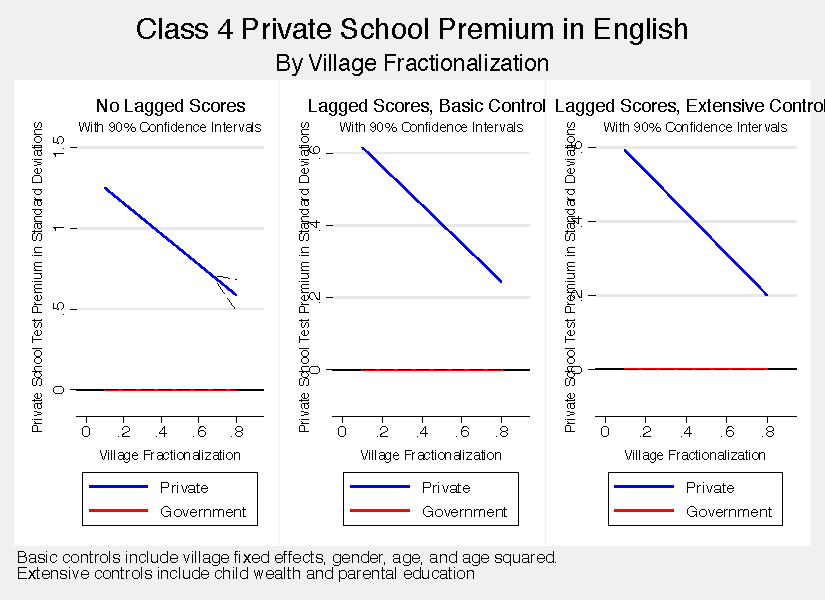
\includegraphics[scale=0.8]{graphs/twoyear_english.pdf} 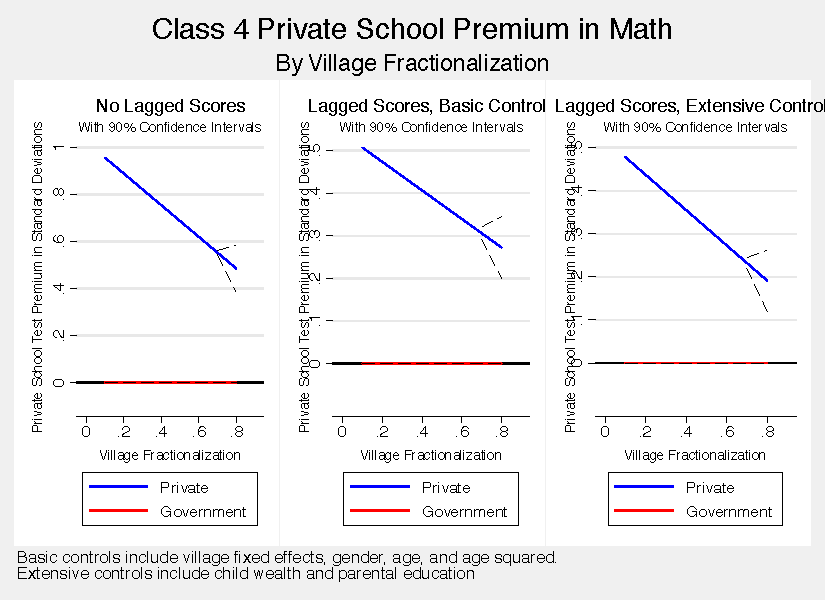
\includegraphics[scale=0.8]{graphs/twoyear_math.pdf}
	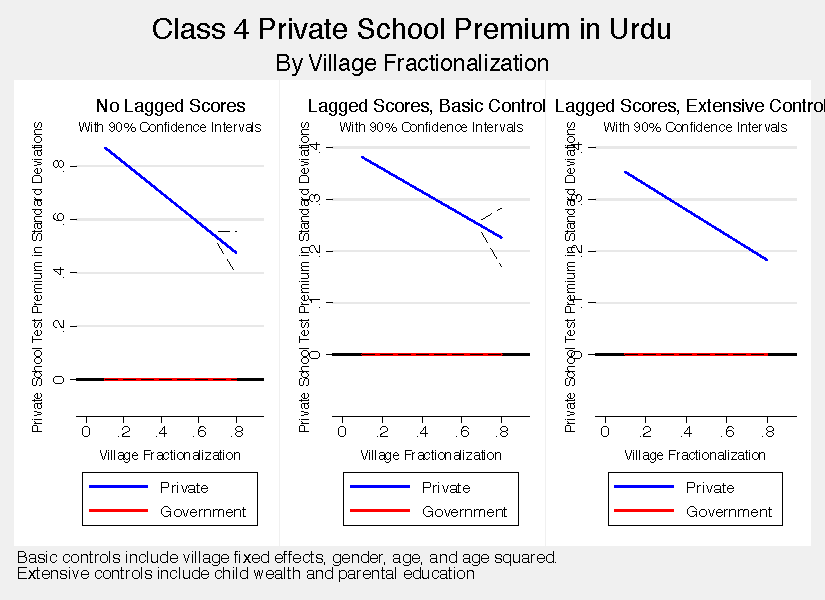
\includegraphics[scale=0.8]{graphs/twoyear_urdu.pdf}
\end{figure}

\begin{sidewaystable}[htbp]\centering
\def\sym#1{\ifmmode^{#1}\else\(^{#1}\)\fi}
\caption{Scores at Class 4\label{wlags}}
\begin{tabular}{l*{9}{c}}
\toprule
                &\multicolumn{3}{c}{English}           &\multicolumn{3}{c}{Urdu}              &\multicolumn{3}{c}{Math}              \\\cmidrule(lr){2-4}\cmidrule(lr){5-7}\cmidrule(lr){8-10}
                &\multicolumn{1}{c}{}&\multicolumn{1}{c}{}&\multicolumn{1}{c}{}&\multicolumn{1}{c}{}&\multicolumn{1}{c}{}&\multicolumn{1}{c}{}&\multicolumn{1}{c}{}&\multicolumn{1}{c}{}&\multicolumn{1}{c}{}\\
\midrule
L.Private School&     1.40***&     0.67***&     0.65***&     0.97***&     0.40***&     0.38***&     1.07***&     0.54***&     0.52***\\
                &  (10.02)   &   (6.52)   &   (5.70)   &   (8.99)   &   (4.74)   &   (4.12)   &   (7.19)   &   (4.54)   &   (4.36)   \\
L.Zaat-Private Interaction&    -0.91***&    -0.53***&    -0.56***&    -0.54***&    -0.22   &    -0.24*  &    -0.63***&    -0.33*  &    -0.41** \\
                &  (-4.19)   &  (-3.52)   &  (-3.41)   &  (-3.14)   &  (-1.63)   &  (-1.68)   &  (-2.66)   &  (-1.86)   &  (-2.29)   \\
Female          &     0.25***&     0.16***&     0.15***&     0.22***&     0.11***&     0.11***&    -0.12** &   -0.075** &   -0.080** \\
                &   (6.81)   &   (6.24)   &   (5.70)   &   (6.62)   &   (4.66)   &   (4.42)   &  (-2.60)   &  (-2.13)   &  (-2.32)   \\
Child Age       &   -0.013   &   -0.025   &   -0.032   &   -0.056   &   -0.026   &   -0.054   &   -0.030   &   -0.029   &   -0.058   \\
                &  (-0.25)   &  (-0.56)   &  (-0.67)   &  (-0.97)   &  (-0.50)   &  (-0.97)   &  (-0.44)   &  (-0.42)   &  (-0.78)   \\
Age Squared     &  0.00010   &  0.00087   &   0.0012   &   0.0013   &  0.00028   &   0.0015   &  0.00025   &  0.00026   &   0.0015   \\
                &   (0.05)   &   (0.45)   &   (0.60)   &   (0.52)   &   (0.12)   &   (0.63)   &   (0.08)   &   (0.09)   &   (0.47)   \\
L.English Theta &            &     0.52***&     0.51***&            &            &            &            &            &            \\
                &            &  (25.05)   &  (24.59)   &            &            &            &            &            &            \\
Child's Wealth Index&            &            &    0.022***&            &            &    0.018***&            &            &    0.033***\\
                &            &            &   (4.73)   &            &            &   (3.92)   &            &            &   (4.98)   \\
Educated Parent &            &            &    0.082***&            &            &    0.083***&            &            &    0.095***\\
                &            &            &   (5.13)   &            &            &   (4.65)   &            &            &   (4.54)   \\
L.Urdu Theta    &            &            &            &            &     0.56***&     0.55***&            &            &            \\
                &            &            &            &            &  (34.73)   &  (34.95)   &            &            &            \\
L.Math Theta    &            &            &            &            &            &            &            &     0.55***&     0.55***\\
                &            &            &            &            &            &            &            &  (29.07)   &  (30.06)   \\
Village Fixed Effects&      Yes   &      Yes   &      Yes   &      Yes   &      Yes   &      Yes   &      Yes   &      Yes   &      Yes   \\
\midrule
Observations    &    14523   &    14523   &    12856   &    14523   &    14523   &    12856   &    14523   &    14523   &    12856   \\
\bottomrule
\multicolumn{10}{l}{\footnotesize \textit{t} statistics in parentheses}\\
\multicolumn{10}{l}{\footnotesize * p<0.10, ** p<0.05, *** p<0.01}\\
\end{tabular}
\end{sidewaystable}


\subsubsection{Value Added}\label{} 
Of course the ``gold-standard'' in education these days is to measure a teacher's ``value-added'', which is computed by regressing each student's current test scores on lagged test scores, a number of controls, and fixed effects for each teacher. The coefficients on these teacher dummies are then extracted and evaluated as the teacher's contribution to student learning (their ``value-added''). 

As shown in Table~\ref{valueadded}, for english and urdu, private school performance is declining as village fractionalization increases (as shown in the columns with district fixed effects), and the gap between government and private schools is declining within villages (as shown in the columns with village fixed effects). 

\begin{sidewaystable}[htbp]\centering
\def\sym#1{\ifmmode^{#1}\else\(^{#1}\)\fi}
\caption{Valued-Added and Village Characteristics\label{valueadded}}
\begin{tabular}{l*{6}{c}}
\toprule
                &\multicolumn{2}{c}{English}&\multicolumn{2}{c}{Math} &\multicolumn{2}{c}{Urdu} \\\cmidrule(lr){2-3}\cmidrule(lr){4-5}\cmidrule(lr){6-7}
                &\multicolumn{1}{c}{District FEs}&\multicolumn{1}{c}{Village FEs}&\multicolumn{1}{c}{District FEs}&\multicolumn{1}{c}{Village FEs}&\multicolumn{1}{c}{District FEs}&\multicolumn{1}{c}{Village FEs}\\
\midrule
Village Fractionalization&     0.60***&            &     0.43*  &            &     0.30** &            \\
                &   (2.90)   &            &   (1.97)   &            &   (2.30)   &            \\
Private School (NGOs set to missing)&     1.10***&     0.83***&     0.40*  &     0.32   &     0.31***&     0.40***\\
                &   (5.92)   &   (4.13)   &   (1.74)   &   (1.38)   &   (2.68)   &   (2.92)   \\
Private School * Village Fractionalization&    -1.04***&    -0.63*  &    -0.43   &    -0.37   &    -0.31*  &    -0.43** \\
                &  (-3.91)   &  (-1.96)   &  (-1.42)   &  (-1.18)   &  (-1.92)   &  (-2.16)   \\
Wealth*: Median Monthly Expenditure& 0.000011   &            & 0.000012   &            &-0.0000076   &            \\
                &   (0.52)   &            &   (0.50)   &            &  (-0.52)   &            \\
dist2           &     0.86***&            &     2.88***&            &     2.15***&            \\
                &  (10.01)   &            &  (28.59)   &            &  (35.23)   &            \\
dist3           &     0.71***&            &     0.38***&            &     1.35***&            \\
                &   (8.15)   &            &   (4.52)   &            &  (22.08)   &            \\
o.Village Fractionalization&            &        0   &            &        0   &            &        0   \\
                &            &      (.)   &            &      (.)   &            &      (.)   \\
\midrule
Observations    &      551   &      551   &      551   &      551   &      551   &      551   \\
\bottomrule
\multicolumn{7}{l}{\footnotesize Weighted by Number of Students}\\
\multicolumn{7}{l}{\footnotesize * p<0.10, ** p<0.05, *** p<0.01}\\
\end{tabular}
\end{sidewaystable}



\section{Alternative Explanations}\label{alts}

\subsection{Changes in Selection?}\label{}
One obvious alternative explanation for the decline of public school test scores is that there is a marked change in the types of students enrolling in private schools. There is little evidence to support this, however. If it were the case that in homogenous villages more talented student attend private schools, but in highly fractionalized villages high caste parents send their children to private schools regardless of latent talent, we would expect to see some change in the degree to which wealth affects school choice. As shown in Figure~\ref{wealthbyfrac} below, however, there is no evidence that such a change has taken place -- the role of wealth in determining school choice appears to be unaffected by village fractionalization.\footnote{This also holds up in regressions.} 

\begin{figure}[htb]
	\begin{center}
	\caption{}\label{wealthbyfrac}
	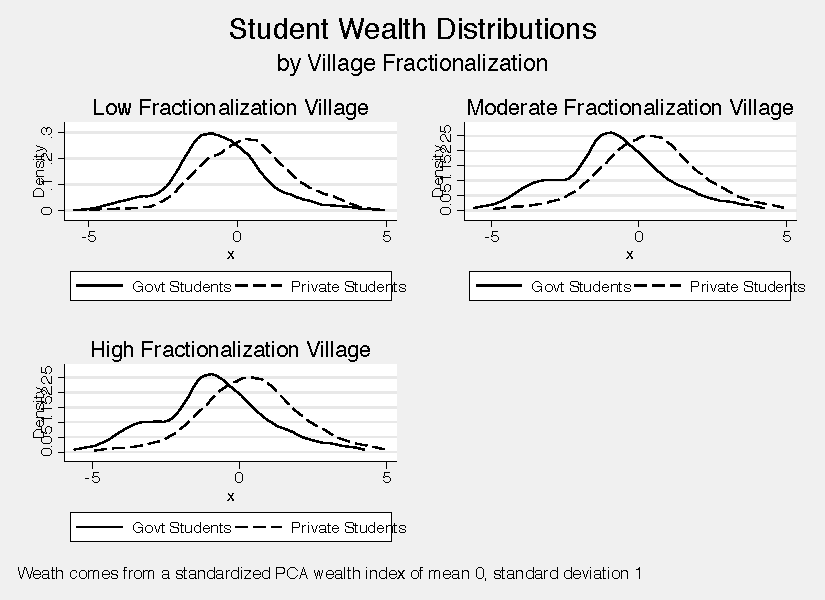
\includegraphics[scale=1.0]{graphs/wealth_by_frac.pdf}
	\end{center}
\end{figure}

\subsection{Differences in Information}\label{}
Another possible explanation for this pattern is that in more ethnically fractionalized villages, parents are less knowledgable about the quality of different schools. This seems a reasonable explanation given how segregated social networks may become in ethnically fractionalized villages. Yet as shown in Table~\ref{knowledge}, there is little evidence for this hypothesis. Measuring ``accuracy of perceptions'' as the correlation between parental rankings of schools (as Excellent, Above Average, Average, Poor, or Very Poor) and objective school ratings (based on average student test scores), we see that there is no systematic difference in awareness of school quality across villages of different level of fractionalization. Similarly, there is no relationship between levels of fractionalization and the share of schools to which parents respond ``don't know'' when asked about school quality. 


\begin{sidewaystable}[htbp]\centering
\def\sym#1{\ifmmode^{#1}\else\(^{#1}\)\fi}
\caption{Parental Knowledge of School Quality\label{knowledge}}
\begin{tabular}{l*{12}{c}}
\toprule
                &\multicolumn{3}{c}{Accuracy, Women}   &\multicolumn{3}{c}{Accuracy, Men}     &\multicolumn{3}{c}{Share of Schools Don't Know, Women}&\multicolumn{3}{c}{Share of Schools Don't Know, Men}\\\cmidrule(lr){2-4}\cmidrule(lr){5-7}\cmidrule(lr){8-10}\cmidrule(lr){11-13}
                &\multicolumn{1}{c}{(1)}&\multicolumn{1}{c}{(2)}&\multicolumn{1}{c}{(3)}&\multicolumn{1}{c}{(4)}&\multicolumn{1}{c}{(5)}&\multicolumn{1}{c}{(6)}&\multicolumn{1}{c}{(7)}&\multicolumn{1}{c}{(8)}&\multicolumn{1}{c}{(9)}&\multicolumn{1}{c}{(10)}&\multicolumn{1}{c}{(11)}&\multicolumn{1}{c}{(12)}\\
                &\multicolumn{1}{c}{English}&\multicolumn{1}{c}{Math}&\multicolumn{1}{c}{Urdu}&\multicolumn{1}{c}{English}&\multicolumn{1}{c}{Math}&\multicolumn{1}{c}{Urdu}&\multicolumn{1}{c}{English}&\multicolumn{1}{c}{Math}&\multicolumn{1}{c}{Urdu}&\multicolumn{1}{c}{English}&\multicolumn{1}{c}{Math}&\multicolumn{1}{c}{Urdu}\\
\midrule
Village         &     0.15   &     0.22   &     0.32   &   -0.042   &    -0.30   &   -0.070   &    0.058   &     0.11   &    0.090   &    0.058   &     0.11   &    0.090   \\
Fractionalization&   (0.45)   &   (0.57)   &   (0.99)   &  (-0.15)   &  (-1.05)   &  (-0.26)   &   (0.81)   &   (1.57)   &   (1.37)   &   (0.81)   &   (1.57)   &   (1.37)   \\
District Fixed Effects &      Yes   &      Yes   &      Yes   &      Yes   &      Yes   &      Yes   &      Yes   &      Yes   &      Yes   &      Yes   &      Yes   &      Yes   \\
\midrule
Observations    &      436   &      411   &      404   &      535   &      540   &      520   &     1437   &     1437   &     1437   &     1437   &     1437   &     1437   \\
\bottomrule
\multicolumn{13}{l}{\footnotesize Accuracy is measured as correlation between 5-fold parental rating of schools and actual school ratings by average score.}\\
\multicolumn{13}{l}{\footnotesize * p<0.10, ** p<0.05, *** p<0.01}\\
\end{tabular}
\end{sidewaystable}



\section{Generalizability}\label{india}
One interesting question is whether the results from this analysis are generalizable. As noted above, the fact that castes are not ordered in a strict hierarchical manner suggests this may be a possibility. 

Although this is obviously HIGHLY preliminary, I examine the private school premium in Indian villages using data from a JPAL education paper. Ethnic fractionalization is estimated using the Indian equivalent of \emph{zaats} -- \emph{jatis}. Unlike the commonly known \emph{varnas} caste divisions (like Brahmin), \emph{jatis} do not have a common hierarchy across villages. These results are SUPER preliminary, and the tests used are much less precise than those used in the LEAPS survey, but all show negative point estimates. Most are not statistically significant, but they are at least suggestive as shown in Tables~\ref{indiareading}-\ref{indiawriting} (I've yet to duplicate the results in the JPAL paper, so this may be wrong...) 


\begin{table}[htbp]\centering
\def\sym#1{\ifmmode^{#1}\else\(^{#1}\)\fi}
\caption{India: Child Reading Skills and Fractionalization\label{indiareading}}
\begin{tabular}{l*{3}{c}}
\toprule
                &\multicolumn{1}{c}{(1)}&\multicolumn{1}{c}{(2)}&\multicolumn{1}{c}{(3)}\\
                &\multicolumn{1}{c}{Read Letters}&\multicolumn{1}{c}{Read Sentence}&\multicolumn{1}{c}{Read Story}\\
\midrule
Private School  &    0.082** &     0.19***&     0.13** \\
                &   (2.57)   &   (3.82)   &   (2.15)   \\
Village Fractionalization&    0.021   &    0.050   &    0.046   \\
                &   (0.59)   &   (1.00)   &   (1.07)   \\
Village Frac * Private&   0.0084   &   -0.030   &    0.090   \\
                &   (0.21)   &  (-0.49)   &   (1.19)   \\
Female          &   -0.049***&    -0.11***&    -0.11***\\
                & (-10.55)   & (-15.70)   & (-16.07)   \\
Child Age       &     0.18***&     0.26***&     0.15***\\
                &  (14.97)   &  (16.12)   &  (11.64)   \\
Child Age Squared&  -0.0069***&  -0.0087***&  -0.0031***\\
                & (-13.04)   & (-12.05)   &  (-5.27)   \\
\midrule
Observations    &    31703   &    31703   &    31703   \\
\bottomrule
\multicolumn{4}{l}{\footnotesize Each model regressions a dummy for given ability against controls}\\
\multicolumn{4}{l}{\footnotesize * p<0.10, ** p<0.05, *** p<0.01}\\
\end{tabular}
\end{table}

\begin{table}[htbp]\centering
\def\sym#1{\ifmmode^{#1}\else\(^{#1}\)\fi}
\caption{India: Child Math Skills and Fractionalization\label{indiamath}}
\begin{tabular}{l*{3}{c}}
\toprule
                &\multicolumn{1}{c}{(1)}&\multicolumn{1}{c}{(2)}&\multicolumn{1}{c}{(3)}\\
                &\multicolumn{1}{c}{Read Numbers}&\multicolumn{1}{c}{Subtraction}&\multicolumn{1}{c}{Division}\\
\midrule
Private School  &     0.17***&     0.16***&     0.11** \\
                &   (3.15)   &   (3.33)   &   (2.31)   \\
Village Fractionalization&    0.010   &    0.069   &    0.085***\\
                &   (0.18)   &   (1.37)   &   (3.19)   \\
Village Frac * Private& -0.00036   &    0.013   &    0.021   \\
                &  (-0.01)   &   (0.20)   &   (0.33)   \\
Female          &    -0.19***&    -0.22***&    -0.19***\\
                & (-25.83)   & (-32.76)   & (-34.18)   \\
Child Age       &     0.24***&     0.14***&    0.079***\\
                &  (16.05)   &  (11.62)   &   (7.59)   \\
Child Age Squared&  -0.0080***&  -0.0041***&  -0.0017***\\
                & (-11.96)   &  (-7.31)   &  (-3.53)   \\
\midrule
Observations    &    31703   &    31703   &    31703   \\
\bottomrule
\multicolumn{4}{l}{\footnotesize Each model regressions a dummy for given ability against controls}\\
\multicolumn{4}{l}{\footnotesize * p<0.10, ** p<0.05, *** p<0.01}\\
\end{tabular}
\end{table}

\begin{table}[htbp]\centering
\def\sym#1{\ifmmode^{#1}\else\(^{#1}\)\fi}
\caption{Child Writing Skills and Fractionalization\label{indiawriting}}
\begin{tabular}{l*{1}{c}}
\toprule
                &\multicolumn{1}{c}{(1)}\\
                &\multicolumn{1}{c}{Can Write Name}\\
\midrule
private==1      &     0.13*  \\
                &   (1.85)   \\
Village Fractionalization&    0.060   \\
                &   (1.41)   \\
(private==1)*panch\_jati\_frac&   -0.052   \\
                &  (-0.60)   \\
Child's sex     &   -0.039***\\
                &  (-6.75)   \\
Lagged Scores   &      Yes   \\
\midrule
Observations    &    15564   \\
\bottomrule
\multicolumn{2}{l}{\footnotesize Each model regressions a dummy for given ability against controls}\\
\multicolumn{2}{l}{\footnotesize * p<0.10, ** p<0.05, *** p<0.01}\\
\end{tabular}
\end{table}



\subsection{Problems}\label{problems}
While I find these results compelling, there are two things that make me slightly uncomfortable. 

First, in most of the paper I have emphasized the declining intra-village test score gap, but a careful reader will of course note that the gap could be declining due to private school decline OR government school improvement. When I drop the village fixed effects, I get differing estimates of the co tribute on of these two tendencies. Cross-sectionally, private scores are relatively flat across villages, and most of the gap closure is coming from improving government schools. When I introduce lagged test scores or do the value added analysis, it's about fifty-fifty. This doesn't terrify me -- I trust those later result much more than the pure cross-section, and if I'm only explaining half the story that's still pretty good. But I cannot for the life of me come up with an explanation for why government schools would be improving with ELF.

The second much more minor issue is that there's nothing fancy in this analysis, which seems a little worrying from an academic politics perspective. I know big names can write papers that just analyze the hell out of surveys, but I'm concerned about putting too much time into something like this if it's likely to be poorly received. I think I'll write it up no matter what -- it's an interesting question -- but guidance as to the amount of time I should invest would be greatly appreciated. 







\end{document}